\documentclass[11pt, a4paper]{article}
\usepackage[utf8]{inputenc}
\usepackage[polish]{babel}
\usepackage{graphicx}
\usepackage[T1]{fontenc}
\usepackage{listings}
\usepackage{hyperref}

\title{
    Temat nr 2 \\
    \textbf{Przewidywanie czasu potrzebnego na dekodowanie filmu} \\
}
\author{Dariusz Hatala, Oxana Danilova}

\begin{document}

\begin{titlepage}
	\centering
	
\includegraphics[width=200pt,height=200pt]{graphics/znak_pk.png}
	\vspace{1cm} \par
	\Large{Politechnika Krakowska} \\
	\vspace{0.2cm} \par
	\Large{Wydział Inżynierii Elektrycznej i Komputerowej}
	\vspace{0.7cm} \par
	\Large{
	    Komputerowe Wspomaganie Decyzji
    }
	\vspace{0.7cm} \par
	\Large{
	    Projekt zaliczeniowy \par
	    zespół nr 2
    }
	\vspace{0.5cm} \par
	\Huge{Ocena czasu potrzebnego na dekodowanie filmu}
	\vspace{1cm} \par
	\Large{
    	\begin{tabular}{c c}
    	    Dariusz Hatala & 31i \\
    	    Oxana Danilova & 31i \\
    	\end{tabular}
	}
    
    \vfill
    
    Pełny kod źródłowy dostępny pod adresem: \url{https://github.com/caspinos/kwd\_ml\_project}
	
	\vfill

	{\large \today\par}
\end{titlepage}

\tableofcontents
\newpage

\section{Cel i zakres projektu}
    Celem projektu jest utworzenie modelu mogącego służyć w celu oceny czasu potrzebnego na transkodowanie filmu z jednego formatu do innego przy jednoczesnej zmianie rozdzelczości.

    \subsection{Źródło danych wejściowych} 
        Dane wejściowe stanowi baza danych: \\
        \textit{Online Video Characteristics and Transcoding Time Dataset Data Set}. \\
        \\
        Dane zostały przygotowane przez \textit{Tewodros Deneke} (tdeneke@abo.fi).
        
    \newpage
    \subsection{Zawartość danych wejściowych}
    
        Dane wejściowe składają się z ponad 68 tyś wpisów zawierających parametry filmów źródłowych i docelowyc oraz czas transkodowania.
        
        Opis poszczególnych danych:
        \begin{description}
            \item [id] Youtube video id
            \item [duration] czas trwania filmu
            \item [bitrate bitrate(video)] bitrate filmu
            \item [height] wysokość filmu w pikselach 
            \item [width] wysokość filmu w pikselach 
            \item [frame rate] framerate filmu
            \item [codec] standard kodowania filmu
            \item [i] liczba klatek typu i (pełne kaltki)
            \item [p] liczba klatek typu p (przewidywana klatka)
            \item [b] liczba klatek typu b (obustronnie przewidywana klatka)
            \item [frames] całkowita liczba klatek
            \item [i\_size] całkowity rozmiar kaltek typu i [bytes]
            \item [p\_size] całkowity rozmiar kaltek typu p [bytes]
            \item [b\_size] całkowity rozmiar kaltek typu b [bytes]
            \item [size] całkowity rozmiar filmu
            \item [o\_codec] wyjściowy kodek
            \item [o\_bitrate] wyjściowy bitrate
            \item [o\_framerate] wyjściowy framerate
            \item [o\_width] wyjściowa szerokość filmu
            \item [o\_height] wyjściowa wysokość filmu
            \item [umem] całkowita ilość pamięci zaalokowana w czasie transkodowania
            \item [utime] całkowity czas transkodowania
        \end{description}

\section{Przygotowanie środowiska}
    Do analizy oraz uczenia maszynowego zostało użyte środowisko Jupyter Notebook oraz język Python 3.
    
    Dodatkowo, wykorzystane zostały następujące biblioteki:
    \begin{itemize}
        \item NumPy (numpy.org)
        \item Pandas (pandas.pydata.org)
        \item Matplotlib (matplotlib.org)
        \item scikit-learn (scikit-learn.org)
        \item Category Encoders (contrib.scikit-learn.org/categorical-encoding)
    \end{itemize}

\newpage
\section{Analiza eksploracyjna danych}
    
\subsection{Ogólne informacje o danych}

    Baza danych zawiera 68784 wierszy oraz 22 kolumny.\\
    Dane nie zawierają brakujący wartości.\\
    Dane nie zawierają zduplikowanych wierszy.\\
    
    Kod użyty do przeprowadzenia analizy:\\
    
        \begin{tabular}{|l|}
            \hline
            \begin{lstlisting}[language=Python]
print(data.shape)
print(data.columns)
            \end{lstlisting}
            \\ \hline
            \begin{lstlisting}[language=Python]
data.head(10)
            \end{lstlisting}
            \\ \hline
            \begin{lstlisting}[language=Python]
data.info()
            \end{lstlisting}
            \\ \hline
            \begin{lstlisting}[language=Python]
data.describe()
            \end{lstlisting}
            \\ \hline
            \begin{lstlisting}[language=Python]
len(data[data.duplicated()])
            \end{lstlisting}
            \\ \hline
        \end{tabular}
    

    \subsection{Badanie korelacji}
    Mapa korelacji ze względu na rozmiar została załączona poza dokumentem (plik \textit{correlations.png}).\par
    Poza oczywistymi zależnościami, można zauważyć, że czas trankodowania jest (liniowo) zależny w znacznym stopniu tylko od parametrów docelowego formatu filmu.\par
    
    \begin{tabular}{|l|}
            \hline
            \begin{lstlisting}[language=Python]
sns.set()

corr = data.sample(1000).corr()

fig, ax = plt.subplots(figsize=(50,30))
sns.heatmap(corr, annot=True, linewidths=.5, ax=ax)
plt.show()
            \end{lstlisting}
            \\ \hline
        \end{tabular}
    
    \newpage
    \subsection{Szczegółowe badanie poszczególnych kolumn numerycznych}
    
    Dla każdej kolumny zostały wyświetlone następujące dane:\par
    \begin{itemize}
        \item nazwa kolumny
        \item liczba unikalnych wartości
        \item histogram
    \end{itemize}

    \begin{tabular}{|l|}
        \hline
        \begin{lstlisting}[language=Python]
numeric_columns = 
        data.select_dtypes(include=np.number).columns
for col in numeric_columns:
print(f'kolumna: {col}')
print(f'unikalnych wartosci: {len(data[col].unique())}')
data[col].plot.hist(bins=40)
plt.show()
        \end{lstlisting}
        \\ \hline
    \end{tabular}\\
    \vspace{0.5cm} 
    
    \textbf{Wnioski:}
    Kolumna 'b\_size' nie zawiera niezerowych wartości. Można ją usunąć. \par
    Kolumna 'b' jest niezerowa w ~1\% przypadków.\par
    Kolumna 'b' jest niezerowy tylko w przypadku użycia kodeka 'h264'.\par
    

    \subsection{Szczegółowe badanie poszczególnych kolumn nienumerycznych}
    
    Dla każdej kolumny zostały wyświetlone następujące dane:\par
    \begin{itemize}
        \item nazwa kolumny
        \item liczba unikalnych wartości
        \item histogram
    \end{itemize}

    \begin{tabular}{|l|}
        \hline
        \begin{lstlisting}[language=Python]
non_numeric_columns 
        = data.select_dtypes(exclude=np.number).columns
for col in non_numeric_columns:
  print(f'kolumna: {col}')
  print(f'unikalnych wartosci: {len(data[col].unique())}')
  if len(data[col].unique()) < 15:
    data[col].value_counts().plot.bar()
    plt.show()
        \end{lstlisting}
        \\ \hline
    \end{tabular}
    
   \newpage 
    \section{Obsługa outlierów}
    
    Do obcięcia outlierów pomocniczo wykorzystujemy poniższe wyznaczniki:
    \begin{equation}
        IQR (interquartile range) = P(75) - P(25) 
    \end{equation} 
    \begin{equation}
        Dolna_granica = P(25) - 1,5*IQR
    \end{equation} 
    \begin{equation}
        Gorna_granica = P(75) + 1,5*IQR
    \end{equation} 
    gdzie P oznacza percentyl. \par
    \vspace{0.5cm}
    Funkcja do wyznaczania powyższych zakresów: \par
    \vspace{0.5cm} 
    
    \begin{tabular}{|l|}
        \hline
        \begin{lstlisting}[language=Python]
def outliners_range(data, column_name):
    rows = data[column_name]
    iqr = np.nanpercentile(rows, 75) - np.nanpercentile(rows, 25)
    lower = (np.nanpercentile(rows, 25) - 1.5*iqr)
    upper = (np.nanpercentile(rows, 75) + 1.5*iqr) 
    return lower, upper
        \end{lstlisting}
        \\ \hline
    \end{tabular}
    \vspace{0.5cm} \\
    
    Dla każdej kolumny zostały przygotowane 2 wykresy:\par
    \begin{itemize}
        \item histogram
        \item wykres pudełkowy
    \end{itemize}\par
    
    \begin{tabular}{|l|}
        \hline
        \begin{lstlisting}[language=Python]
for column in numeric_data:
  print(f'Kolumna: {column}')
  numeric_data[column].plot.hist()
  plt.show()
  numeric_data[column].plot.box()
  plt.show()
        \end{lstlisting}
        \\ \hline
    \end{tabular}
    \vspace{0.5cm} \\
    
    \newpage
    \subsubsection{Kolumna 'frames'}
    
    lower, upper = (-7805.5, 19454.5)\\
    wartości >19454.5: 3076 (4.47\%)\\
    wartości >30k: 869 (1.26\%)\\
    wartości >35k: 20 (0.03\%)\\
    \vspace{0.5cm} \\
    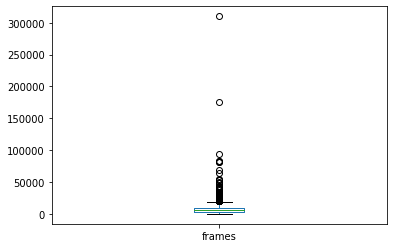
\includegraphics[height=170pt]{graphics/frames_before.png}
    \vspace{0.5cm} \\
    Zdecydowaliśmy się na usunięcie wierszy z wartościami frames > 35000\\
    
    \vspace{0.5cm} 
    \begin{tabular}{|l|}
        \hline
        \begin{lstlisting}[language=Python]
 data_2 = data_2[data_2['frames'] <= 35000 ]
        \end{lstlisting}
        \\ \hline
    \end{tabular}
    \vspace{0.5cm} \\
    
    Po usunięciu:\\
    
    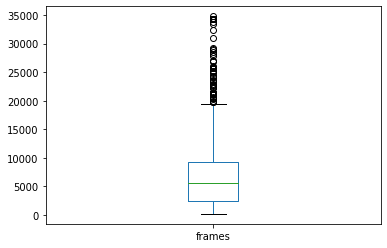
\includegraphics[height=170pt]{graphics/frames_after.png}

    \newpage
    \subsubsection{Kolumna 'duration'}

    lower, upper = (-302.0675, 788.1525)\\
    wartości >788: 3080 (4.48\%)\\
    wartości >1000: 1718 (2.5\%)\\
    wartości >1500: 865 (1.26\%)\\
    wartości >2000: 13 (0.02\%)\\

    \vspace{0.5cm} 
    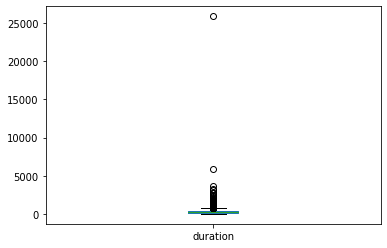
\includegraphics[height=170pt]{graphics/duration_before.png}
    \vspace{0.5cm} \\
    
    Zdecydowaliśmy się na usunięcie wierszy z wartościami duration > 2000
    
    \vspace{0.5cm} 
    \begin{tabular}{|l|}
        \hline
        \begin{lstlisting}[language=Python]
data_2 = data_2[data_2['duration'] <= 2000 ]
        \end{lstlisting}
        \\ \hline
    \end{tabular}
    \vspace{0.5cm} \\
    
    Po usunięciu:\\
    
    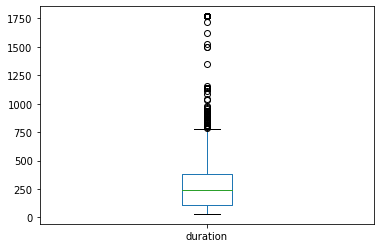
\includegraphics[height=170pt]{graphics/duration_after.png}
    
    \section{Feature engineering}
\subsection{Dodatkowe pole 'pixels'}
    \vspace{0.5cm} 
    \begin{tabular}{|l|}
        \hline
        \begin{lstlisting}[language=Python]
data_3['pixels'] = data_3['width'] * data_3['height']
        \end{lstlisting}
        \\ \hline
    \end{tabular}
    \vspace{0.5cm} \\

\subsection{Dodatkowe pole 'o\_pixels'}
    \vspace{0.5cm} 
    \begin{tabular}{|l|}
        \hline
        \begin{lstlisting}[language=Python]
data_3['o_pixels'] = data_3['o_width'] * data_3['o_height']
        \end{lstlisting}
        \\ \hline
    \end{tabular}
    \vspace{0.5cm} \\

\section{Feature selection - usunięcie zbędnych kolumn}

Zdecydowaliśmy usunąć następujące pola:
\begin{itemize}
\item pole id
\item pole b\_size (brak niezerowych wartości)
\item pole umem (nie podlegająca analizie wartość wynikowa )
\end{itemize}

    \vspace{0.5cm} 
    \begin{tabular}{|l|}
        \hline
        \begin{lstlisting}[language=Python]
data_4 = data_4.drop(['id', 'b_size', 'umem'], axis=1)
        \end{lstlisting}
        \\ \hline
    \end{tabular}
    \vspace{0.5cm} \\

\newpage
\section{Data Preparation - przygotowanie danych do uczenia}
\subsection{Kodowanie pól kategorycznych}
    \vspace{0.5cm} 
    \begin{tabular}{|l|}
        \hline
        \begin{lstlisting}[language=Python]
categorical_cols = ['codec', 'o_codec']

ohe = ce.OneHotEncoder(cols=categorical_cols, return_df=True, 
        use_cat_names=True, handle_unknown=0)
data_5 = ohe.fit_transform(data_5)
        \end{lstlisting}
        \\ \hline
    \end{tabular}
    \vspace{0.5cm} \\

\subsection{Podział danych na wejściowe i wynikowe }

    \vspace{0.5cm} 
    \begin{tabular}{|l|}
        \hline
        \begin{lstlisting}[language=Python]
target = data_5['utime']
features = data_5.drop('utime', axis=1)
        \end{lstlisting}
        \\ \hline
    \end{tabular}
    \vspace{0.5cm} \\

\subsection{Skalowanie danych}

    \vspace{0.5cm} 
    \begin{tabular}{|l|}
        \hline
        \begin{lstlisting}[language=Python]
from sklearn.preprocessing import MinMaxScaler

scaler = MinMaxScaler()
features_scaled = scaler.fit_transform(features)
        \end{lstlisting}
        \\ \hline
    \end{tabular}
    \vspace{0.5cm} \\

\subsection{Podział danych na trenujące i testujące}

    \vspace{0.5cm} 
    \begin{tabular}{|l|}
        \hline
        \begin{lstlisting}[language=Python]
X_train, X_test, y_train, y_test = 
		train_test_split(
        		features_scaled, 
        		target, 
        		test_size=0.3, 
        		random_state=0)
        \end{lstlisting}
        \\ \hline
    \end{tabular}
    \vspace{0.5cm} \\

\newpage
\section{Trenowanie oraz ewaluacja modeli}
Ewaluacja oraz porównanie modeli bazuje na błędzie średnio-kwadratowym oraz parametrze R2.

\subsection{Podstawowy model regresji liniowej}
    \vspace{0.5cm} 
    \begin{tabular}{|l|}
        \hline
        \begin{lstlisting}[language=Python]
lr = LinearRegression()
lr.fit(X_train, y_train)

print("Mean squared error of a linear model: %.2f" % 
      mean_squared_error(y_test, lr.predict(X_test)))
score = lr.score(X_test, y_test) #r2_score
print("Linear Regression R2 score: %.2f" % score)
        \end{lstlisting}
        \\ \hline
    \end{tabular}
    \vspace{0.5cm} \\

\textbf{Wyniki:}\\
Mean squared error of a linear model: 124.55\\
Linear Regression R2 score: 0.53\\

\subsection{Wyszukiwanie optymalnego modelu z wykorzystaniem Polynominal Features, ElasticNet oraz GridSearch}

    \vspace{0.5cm} 
    \begin{tabular}{|l|}
        \hline
        \begin{lstlisting}[language=Python]
parameters=[{
     'alpha':[0.1, 0.2, 0.5, 0.9], 
     'l1_ratio':[0.1, 0.2, 0.5, 0.9],
     }
]
 
for pf_level in range(1,3):
    print(f"polynominal features level {pf_level}:")

    pf = PolynomialFeatures(pf_level)
    train_poly = pf.fit_transform(X_train)
    test_poly  = pf.fit_transform(X_test)
    
    model = GridSearchCV( ElasticNet(), parameters, cv=5 )
    model.fit(train_poly, y_train)

    print(f"  {model.best_estimator_}")
    print("    Mean squared error: %.2f" % 
    mean_squared_error(y_test, model.predict(test_poly)))
    score = model.score(test_poly, y_test) #r2_score
    print("    R2 score: %.2f" % score)
        \end{lstlisting}
        \\ \hline
    \end{tabular}
    \vspace{0.5cm} \\
    
    \textbf{Wyniki:}\\
 \begin{verbatim}
polynominal features level 1:
  ElasticNet(alpha=0.1, copy_X=True, fit_intercept=True, l1_ratio=0.9,
           max_iter=1000, normalize=False, positive=False, precompute=False,
           random_state=None, selection='cyclic', tol=0.0001, warm_start=False)
    Mean squared error: 127.97
    R2 score: 0.52
polynominal features level 2:
  ElasticNet(alpha=0.1, copy_X=True, fit_intercept=True, l1_ratio=0.9,
           max_iter=1000, normalize=False, positive=False, precompute=False,
           random_state=None, selection='cyclic', tol=0.0001, warm_start=False)
    Mean squared error: 57.47
    R2 score: 0.78
\end{verbatim}

\subsection{Podsumowanie}
Przy użyciu cech wielomianowych oraz optymalizacji parametrów udało nam się znacząco zwiększyć dokładność modelu.

\end{document}


